\documentclass{article}

% Language setting
% Replace `english' with e.g. `spanish' to change the document language
\usepackage{biblatex} %Imports biblatex package
\usepackage{tikz}
\usetikzlibrary{trees}
\addbibresource{sample.bib}
\usepackage[english]{babel}
\usepackage{array}
\usepackage{amsmath}
\usepackage{pythonhighlight}
\newcolumntype{P}[1]{>{\centering\arraybackslash}p{#1}}
\newcolumntype{M}[1]{>{\centering\arraybackslash}m{#1}}

% Set page size and margins
% Replace `letterpaper' with `a4paper' for UK/EU standard size
\usepackage[letterpaper,top=2cm,bottom=2cm,left=3cm,right=3cm,marginparwidth=1.75cm]{geometry}

\usepackage{amsmath}
\usepackage{graphicx}
\usepackage[colorlinks=true, allcolors=blue]{hyperref}
\usepackage{setspace}
\usepackage{booktabs}
\usepackage[T1]{fontenc}
\usepackage{longtable}
\doublespacing

\begin{document}
\tikzstyle{every node}=[draw=black,thick,anchor=west]
\tikzstyle{selected}=[draw=red,fill=red!30]
\tikzstyle{optional}=[dashed,fill=gray!50]
\begin{titlepage}

\centering
\scshape
\vspace{\baselineskip}

%
\rule{\textwidth}{1.6pt}\vspace*{-\baselineskip}\vspace*{2pt}
\rule{\textwidth}{0.4pt}

{\Huge \textbf{\textsc{NPRE 449: Homework 3 \\
\vspace{15pt}}}}

\rule{\textwidth}{0.4pt}\vspace*{-\baselineskip}\vspace{3.2pt}
\rule{\textwidth}{1.6pt}\vspace{6pt}
%%\centerline{\textit{University of Illinois at Urbana-Champaign}} 
\vspace{1.5\baselineskip}


\large \centerline{\textbf{Author:} Nathan Glaser}
\large \centerline{\textbf{Net-ID:} nglaser3}
\quad

\vfill
\large \centerline{September 18, 2024}
%
\pagenumbering{gobble}
\end{titlepage}

\tableofcontents
\newpage
\pagenumbering{arabic}

\section*{Question 1}
\addcontentsline{toc}{section}{\protect\numberline{}Question 1}

For starters, lets analyze fission. Fission occurs when a fissile/fissionable atom absorbs a neutron (or spontaneously fissions), splitting the atom apart. Not every absorption reaction yields a fission event. In 'thermal' nuclear reactors, we rely on thermal or low-energy neutrons to induce fission events. Each fission event typically produces multiple products: 2 (or more) fission fragments, neutrinos, prompt gammas, and prompt neutrons. Each fission reaction typically releases roughly 200 MeV. From here, each fission fragment, depending on which isotopes are produced, have the potential to decay, and likely will. Each decay will produce either a delayed neutron, delayed gamma, a beta, or sometimes alphas --- though we don't really care about alphas --- and a daughter nuclide. This daughter nuclides typically also decays. Delayed neutrons have the potential of causing further fissions, or be parasitically captured. Similarly, prompt neutrons can induce a fast fission event, be parasitically absorbed, or also in/elastically scatter. Gamma rays and beta rays can also potentially be absorbed. The neutrinos released do not interact with anything. Scatter/absorption events excite nuclei, often inducing a decay event, if not a release of energy in the form of a gamma ray. An event tree is presented in Fig. \ref{fig:tree} for reference, although it should be noted this tree only goes two events down, and does not show the loops occurring from potential fissions. Finally, Table \ref{tab:breakdown} shows each form of energy release and their share of the total energy release. 

\vspace{2cm}

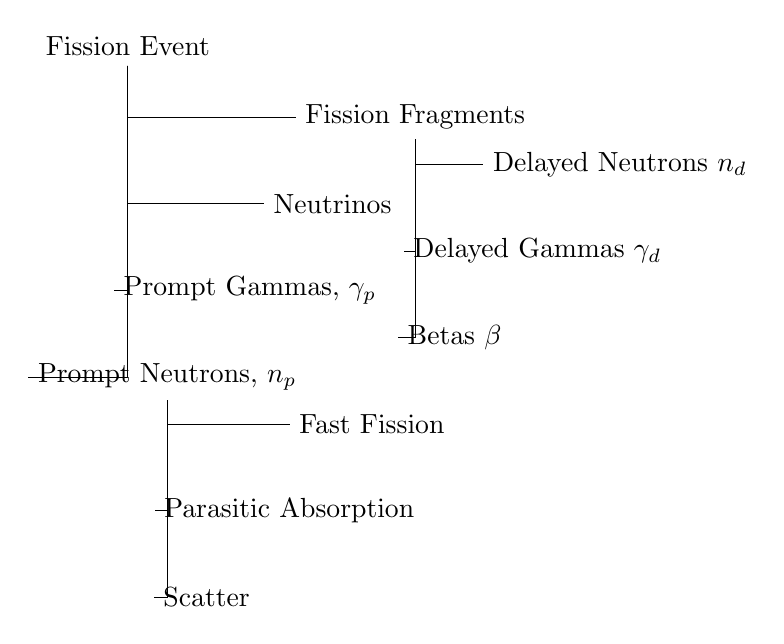
\begin{tikzpicture}[%
  grow via three points={one child at (.5,-.0) and
  two children at (1.55,-.3) and (0.5,-1.4)},
  edge from parent path={(\tikzparentnode.south) |- (\tikzchildnode.west)}]
  \node {Fission Event}
    child { node {Fission Fragments}
        child { node {Delayed Neutrons $n_d$}}
        child { node {Delayed Gammas $\gamma_d$}}
        child { node {Betas $\beta$}}}
    child { node {Neutrinos} }
    child { node {Prompt Gammas, $\gamma_p$}}
    child { node {Prompt Neutrons, $n_p$}
        child { node {Fast Fission}}
        child { node {Parasitic Absorption}}
        child { node {Scatter}}};
\label{fig:tree}
\end{tikzpicture}

\begin{table}[]
    \centering
    \def\arraystretch{1.5}
    \caption{Breakdown of energy released in a nuclear reactor}
    \begin{tabular}{|c|c|c|c|}
        \hline
        Time Scale & Particle Type & Percent Share & Deposition Location\\
        \midrule
        \hline
        & Fission Fragments & 80.5 & Fuel\\
        Instantaneous & Neutrinos & 5.0 & Non-Recoverable \\
        & Prompt Gamma Rays & 2.5 &  High Z --- Fuel / Structures\\
        & Prompt Neutrons & 2.5 & Moderator\\
        \midrule
        \hline
        & Delayed Neutrons & 0.02 & Fuel / Moderator\\
        Delayed & Beta Decay & 2.5  & Fuel\\
        & Delayed Gamma Rays & 3.0 & High Z --- Fuel / Structures\\
        \midrule
        \hline
        &&&\\
        Both & Parasitic Absorptions & 3.5 & Fuel / Structures\\
        &&&\\
        \hline
    \end{tabular}
    \label{tab:breakdown}
\end{table}

\end{document}